\section{Estado del arte}
\label{sec:StateOfTheArt}


\subsubsection{Eventos}

Los frameworks que se manejan con eventos resuelven estos problemas 

1) A 'mano' como los frameworks que implementan la interfaz Javabeans (Arena
actual | SWT )\\ 


{\bf JavaBeans} representa una implementación del módelo Propiedad-Evento-Método

Un componente JavaBean se define a través de :

\begin {itemize}

\item Las propiedades que expone.
\item Los métodos que ofrece.
\item Los eventos que atiende o genera.

\end {itemize}

Para gestionar estas características, todo JavaBean debe ofrecer:

\begin {itemize}

\item {\bf Soporte para Introspeción:} El bean tiene que ofrecer la
información necesaria para que la herramienta de diseño pueda analizar sus características de forma opaca.

\item {\bf Soporte para Customización:} La herramienta de construcción de la
aplicación puede adaptar (“customizar”) la apariencia o comportamiento del bean a la  aplicación.

\item {\bf Soporte para Persistencia:} El estado de un bean customizado puede
ser almacenado para ser utilizado más tarde.

\item {\bf Soporte para Eventos:} Los beans se comunican a través del envío y
	  recepción de eventos.

\end {itemize}

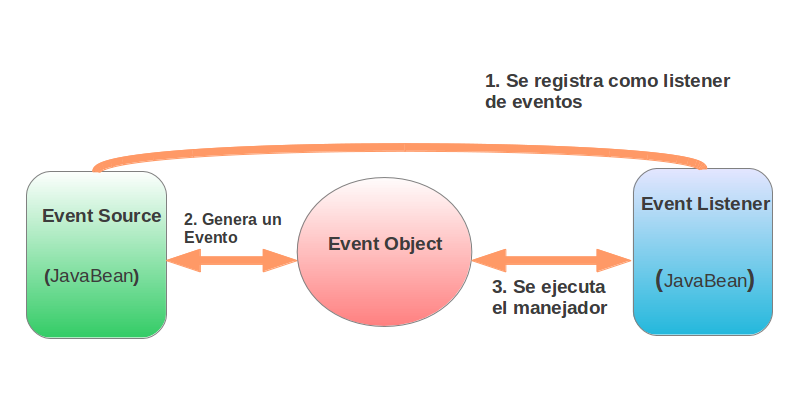
\includegraphics[width=350px, height=200px]{img/javabeans}


{\bf wicket} Es un Framework web MVC para Java.\\
El Sistema de binding de wichet es atravez de submit de un formulario.
Desventajas.
\begin {itemize}

\item Las validaciones del dominio solo se hacen cuando en el submit.

\item Incorporar el concepto de Form.

\end {itemize}

3) investigar que hace morphic




\subsubsection{Transacciones}

{\bf Soluciones comunes:}

\begin {itemize}

\item Patron: Objectos de transaccion
\item Unidad de trabajo
\item Clonar al editar
\item Transacciones de Base de datos 
\end {itemize}

\begin {itemize}

\item {\bf Objetos de transaccion}
Provee una interfaz separada para las transacciones en el contexto de capas de
acceso a bases de datos.\\
{\bf Solucion} Utilizar un objeto de transaccion. Hay que hacer rollback en el
destructor, para que las transacciones abiertas sean abortadas.

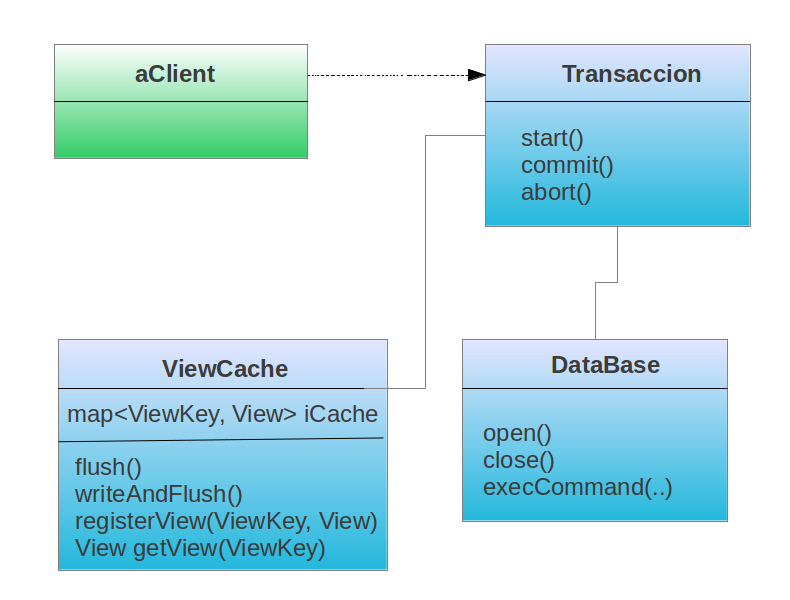
\includegraphics[width=300px, height=200px]{img/objectTransaction}

\item {\bf Unidad de tranajo }
Mantiene una lista de objetos afectados por una transaccion de negocio y
coordina los cambios de escritura y la resolucion de problemas de concurrencia.
Una unidad de trabajo realiza un seguimiento de todo lo que haces durante una
transacción que puede afectar a la base de datos. 
Cuando haya terminado,impacta todos los cambios en la base de datos.

\item {\bf Clonar al editar}
Esta solucion es bastante comúm. En el momento que se quiere editar un objeto,
se lo clona, y se modifica el objeto clonado. Cuando se confima la edicion, se
impacta los cambios del clon en el objeto original.

\item {\bf Transacciones de base de datos}
Con este sistema, al momento de edicion del objeto, se crea una transaccion en
la base de datos, y en la confirmacion de la edicion, se comitea la transaccion.
Y si se quiere cancelar, se hace un rollback en la transaccion y los cambios se
revierten.

\end {itemize}

